\documentclass{article}

\usepackage[dutch]{babel}
\usepackage[margin=3cm]{geometry}
\usepackage{graphicx}
\usepackage{float}
\usepackage{caption}
\usepackage{hyperref}
\usepackage{amsmath}
\usepackage{wrapfig}
\usepackage[parfill]{parskip}

% fonts
\usepackage[T1]{fontenc}
\usepackage{helvet}
\renewcommand{\familydefault}{\sfdefault}

\graphicspath{{img/}}

% theorem environment
\usepackage{amssymb}

\newtheorem{theorem}{Definitie}[section]

\usepackage{enumitem}

\newenvironment{thmenum}
 {\begin{enumerate}[label=\upshape\bfseries(\roman*)]}
 {\end{enumerate}}

\usepackage{minted}
\usepackage{upquote}
\usepackage{color}

\begin{document}

\begin{titlepage}
    \author{Tuur Vanhoutte}
    \title{Backend Development}
\end{titlepage}

\pagenumbering{gobble}
\maketitle
\newpage
\tableofcontents
\newpage

\pagenumbering{arabic}

\section{.Net Core \& Web API}

\subsection{.NET Historiek}

\subsubsection{.NET Framework}

\begin{itemize}
    \item Ontwikkeling .NET Framework \& C\# begonnen einde Jaren 90 (Opkomst van Java, Microsoft moest reageren $\Rightarrow$ C\#)
    \item Versie 1.0 .NET Framework op 13 February 2002
    \item Windows Only
    \begin{itemize}
        \item Beperkt open source via Home | Mono (\url{mono-project.com})
    \end{itemize}
    \item Was vooral framework voor desktop applicaties (Winforms, WPF)
    \item Web applicaties via ASP.NET Forms
    \item Laatste versie .NET Framework is 4.8 (april 2019)
    \item Geen verdere ontwikkeling meer van .NET Framework
\end{itemize}

\subsubsection{Rond 2012 enkel strategische veranderingen}

\begin{itemize}
    \item Dominantie Windows was minder groot geworden
    \begin{itemize}
        \item Opkomst mobile devices (iPhone, Android)
        \item Cloud was belangrijker aan het worden (veel Linux)
        \item Open-source werd belangrijker
    \end{itemize}
    \item Microsoft zag een shift van .NET Framework naar andere technologie (Node, Python, etc\dots)
\end{itemize}

\subsubsection{Ontwikkeling .NET Core}

\begin{itemize}
    \item Cross platform (Windows/Linux/macOS)
    \item Volledig open-source
    \begin{itemize}
        \item Samsung TV
        \item ARM Raspberry Pi
        \item \dots
    \end{itemize}
    \item Clean-up van bestaande .NET Framework code
    \item Zoveel mogelijk compatibel
    \item Built for the Cloud
\end{itemize}

Sinds November 2020 spreken we niet meer over .NET Framework of .NET Core maar over .NET 5, .NET 6, .NET 7, \dots

\subsubsection{Tijdslijn}

\begin{itemize}
    \item .NET 5 $\Rightarrow$ November 2020
    \item .NET 6 $\Rightarrow$ November 2021 (LTS)
    \item .NET 7 $\Rightarrow$ November 2022
    \item .NET 8 $\Rightarrow$ November 2023 (LTS)
    \item LTS $\Rightarrow$ 3 jaar support
    \item Zonder LTS $\Rightarrow$ 1 jaar support
\end{itemize}

Alles volledig opensource via \url{https://github.com/dotnet}

\subsection{Soorten .NET applicaties}

\subsubsection{Type applicaties in .NET 5:}

\begin{itemize}
    \item ASP.NET Web Applicaties
    \item Console Applicaties
    \item Xamarin
    \item Winforms \& WPF Desktop applicaties
\end{itemize}

\subsubsection{Ondersteuning voor verschillende talen}

\begin{itemize}
    \item C\# (wij gebruiken dit)
    \item Visual Basic
    \item F\# (functional programming)
    \item C++ (desktop development)
\end{itemize}

\subsubsection{Toekomst desktop development}

\begin{itemize}
    \item Zeker nog belangrijk
    \item Niet alles kan in de browser (vb zware 3D apps, interfacing met machines etc)
    \item Zit niet meer in MCT opleiding (wel Xamarin natuurlijk)
    \item Project MAUI
    \begin{itemize}
        \item 1 framework voor .NET/Xamarin/Windows Desktop
        \item Introducing .NET Multi-platform App UI | .NET Blog : \url{https://devblogs.microsoft.com/dotnet/introducing-net-multi-platform-app-ui/}
    \end{itemize}
\end{itemize}

\subsection{ASP.NET Core}

= Framework voor het bouwen van Web Applicaties

\subsubsection{Verschillende soorten applicaties zijn mogelijk:}

\begin{itemize}
    \item Klassieke server-side framework (Razor) (zoals PHP,...)
    \item Realtime Framework (web sockets etc...) met als naam Signal R
    \item Frontend Framework Blazor (C\# in de browser)
    \begin{itemize}
        \item Web Assembly support
    \end{itemize}
    \item \textbf{Framework om API’s te bouwen , webapi (wij gebruiken dit)}
\end{itemize}

Cross platform zowel om uit te voeren als te onwikkelen (Visual Studio \& Visual Studio Code zijn cross-platform)

\subsubsection{ASP.NET Web API}

= Framework voor het bouwen van API’s voor toepassingen

Deze toepassingen zijn:

\begin{itemize}
    \item Front-End Web App (Vue, Angular, Blazor,...)
    \item Desktop Applications
    \item Alles wat HTTP calls kan uitvoeren en JSON begrijpt
\end{itemize}

Zelfde als HTTP Triggers in Azure Functions (cfr. Module IoT Cloud Semester 3)

\subsection{HTTP (Herhaling)}

= Hyper Tekst Transfer Protocol

\begin{itemize}
    \item Onderliggende protocol waarop Internet werkt
    \item Opvragen van tekst, bestanden vanaf servers
    \item Request \textit{meestal} afkomstig van een webbrowser maar ook smartphone, IoT device
    \item HTTP zal bepalen hoe een request en response er moeten uitzien
    \item HTTP bevat een aantal commando’s (HTTP Verbs)
    \item HTTP is stateless, het zal dus geen rekening houden met voorgaande requests
    \item HTTP is niet sessionless, we kunnen cookies (client-side) gebruiken om data bij te houden
    \item HTTP is relatief eenvoudig
\end{itemize}

\subsection{API Design}

\begin{itemize}
    \item In deze module gaan we API's programmeren
    \item De bedoeling is dat frontend applications deze gebruiken
    \item Onze API's zullen enkel JSON data ontvangen en terugsturen
    \item Oudere API's systemen keren soms ook XML terug (deze zien wij niet)
    \item Een API noemen we ook soms een endpoint
    \item De vorm en naamgeving is hier belangrijk
\end{itemize}

\subsubsection{Richtlijnen bij het opstellen van API URL's}

\begin{itemize}
    \item Gebruik Engelse woorden
    \item Start met het woord `api':
    \begin{itemize}
        \item http://www.mct.be/\textcolor{red}{api}
    \end{itemize}
    \item In de URL plaatsen we de naam van objecten die we wensen op te halen
    \begin{itemize}
        \item http://www.mct.be/api/\textcolor{red}{courses}
    \end{itemize}
    \item Willen we specieke cursus ophalen op basis van zijn code steken we dit in de URL
    \begin{itemize}
        \item http://www.mct/be/api/courses/\textcolor{red}{MCT2IOTCLOUD}
    \end{itemize}
    \item Willen we de weken ophalen, plaatsen we dit ook in de URL
    \begin{itemize}
        \item http://www.mct/be/api/courses/MCT2IOTCLOUD/\textcolor{red}{weeks}
    \end{itemize}
    \item Zoeken in de weken kunnen we als volgt gaan doen:
    \begin{itemize}
        \item http://www.mct/be/api/courses/MCT2IOTCLOUD/weeks\textcolor{red}{?q=iothub}
    \end{itemize}
    \item Wil je een bepaalde week ophalen:
    \begin{itemize}
        \item http://www.mct/be/api/courses/MCT2IOTCLOUD/weeks/\textcolor{red}{1}
    \end{itemize}
    \item Wil je de docent ophalen kan dit op deze manier in de URL:
    \begin{itemize}
        \item http://www.mct/be/api/courses/MCT2IOTCLOUD/weeks/1/\textcolor{red}{teacher}
    \end{itemize}
\end{itemize}

\subsection{Anatomie van een ASP.NET Web API Project}

\subsubsection{csproj file}

\begin{figure}[H]
    \centering
    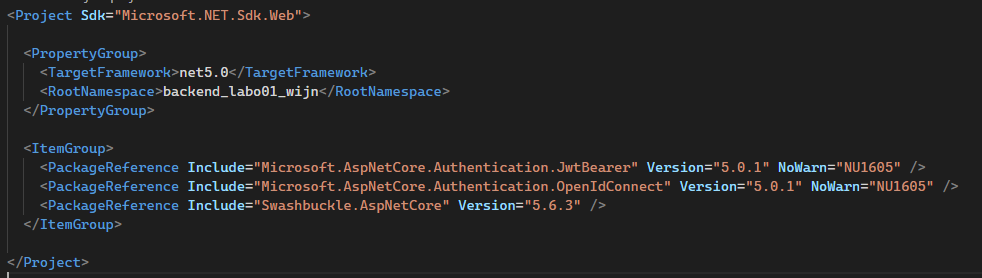
\includegraphics[width=0.5\textwidth]{csproj.png}
    \caption{csproj voorbeeld}
\end{figure}

\begin{itemize}
    \item Beschrijft project
    \item Zal ingelezen worden door Visual Studio
    \item Bevat alle referenties naar gebruikte nuget packages
    \item dotnet build etc zal deze file gebruiken
    \item We mogen deze wijzigen (maar weet wat je doet)
\end{itemize}



\subsubsection{Program.cs}

\begin{itemize}
    \item Main entry point van ASP.NET API applicatie
    \item Hier begint alles
    \item Soms moeten we hier iets instellen
    \item Voorlopig niet van belang
\end{itemize}

\subsubsection{Startup.cs}

\begin{itemize}
    \item Naam spreekt voor zich, bevat alle startup code voor onze API
    \item Hier bepalen we welke \textbf{services} we wensen te gebruiken van ASP.NET 
        
        
\end{itemize}

\begin{figure}[H]
    \centering
    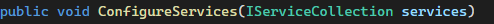
\includegraphics[width=0.7\textwidth]{startup-cs1.png}
    \caption{ConfigureServices}
\end{figure}
\begin{figure}[H]
    \centering
    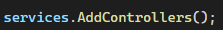
\includegraphics[width=0.4\textwidth]{startup-cs2.png}
    \caption{Controllers}
\end{figure}
\begin{figure}[H]
    \centering
    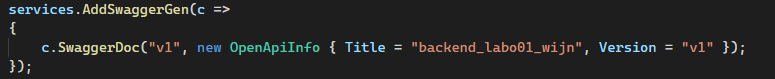
\includegraphics[width=0.6\textwidth]{startup-cs3.png}
    \caption{Swagger}
\end{figure}

\begin{theorem}[Dependency Injection]

Dependency Injection is het injecteren van services in de ASP.NET Container

(komen we later nog op terug)
\end{theorem}

\begin{figure}[H]
    \centering
    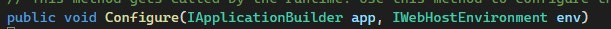
\includegraphics[width=0.7\textwidth]{startup-cs4.png}
    \caption{Configureren van de HTTP Pipeline}
\end{figure}
\begin{figure}[H]
    \centering
    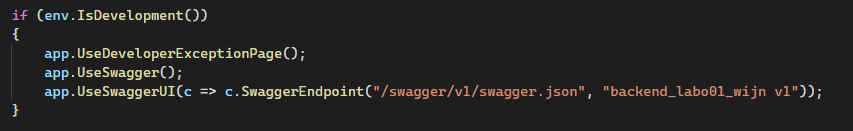
\includegraphics[width=0.6\textwidth]{startup-cs5.png}
    \caption{Configureren van services}
\end{figure}
\begin{figure}[H]
    \centering
    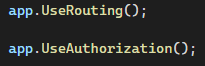
\includegraphics[width=0.3\textwidth]{startup-cs6.png}
    \caption{Configureren van Routing, Security etc\dots}
\end{figure}


\textbf{HTTP Pipeline}

\begin{itemize}
    \item We spreken van middleware componenten in de pipeline
    \item Deze componenten zijn verbonden en geven de data door aan elkaar
    \item Ieder component zal zijn bijdrage leveren
    \item Endpoint is onze code in de controller
    \item Request en Response gaan door deze pipeline
    \item ASP.NET Core Middleware: \url{https://docs.microsoft.com/en-us/aspnet/core/fundamentals/middleware/?view=aspnetcore-5.0}
\end{itemize}

\begin{figure}[H]
    \centering
    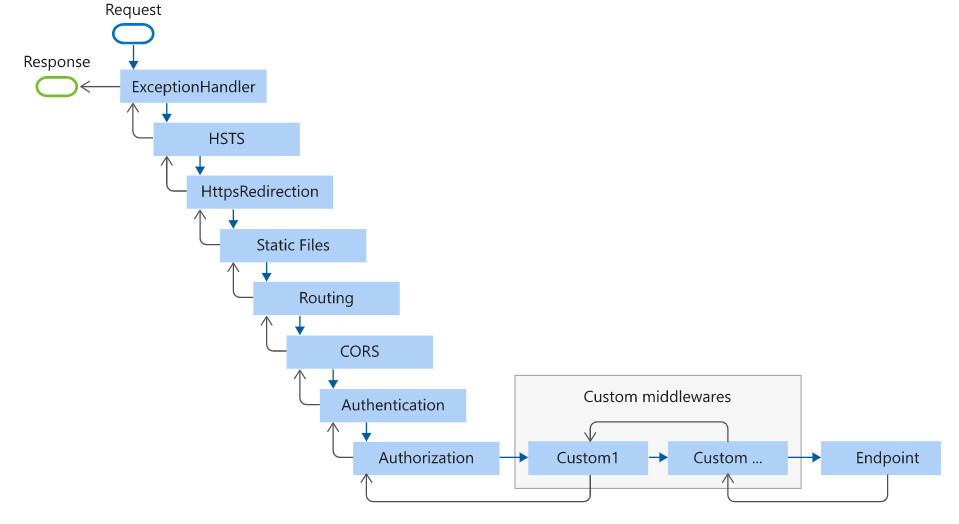
\includegraphics[width=0.7\textwidth]{http-pipeline.png}
    \caption{De HTTP Pipeline met middleware componenten}
\end{figure}

\subsubsection{Appsetting.json}

= Configuratie info nodig in de applicatie

\begin{itemize}
    \item Niet inchecken in GitHub (.gitignore gebruiken)
    \item Bv.: Mailserver settings, connectionstrings etc...
    \item We zien later (in een labo) hoe we deze kunnen uitlezen
    \item We kunnen verschillende files gebruiken:
    \begin{itemize}
        \item Appsettings.Development.json
        \item Appsettings.Production.json
        \item \dots
    \end{itemize}
    \item Configuration in ASP.NET Core: \url{https://docs.microsoft.com/en-us/aspnet/core/fundamentals/configuration/?view=aspnetcore-5.0}
\end{itemize}

\subsection{Controllers}

\begin{itemize}
    \item Belangrijkste concept in ASP.NET
    \item Zorgt voor de verwerking van de requests
    \item Zal een response terugkeren naar de aanvrager (bv. onze React JS applicatie)
    \item Is klasse in map \textbf{Controllers} in onze applicatie
    \item Naam moet eindigen op \textbf{Controller}
    \item Klasse moet erven van \textbf{ControllerBase}
    \item Attribute [ApiController] moet er staan om aan te duiden dat het een API is als we [Route] gebruiken op Controller niveau
    \item Via [Route] kunnen we de URL bepalen
\end{itemize}

\begin{figure}[H]
    \centering
    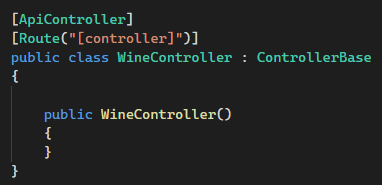
\includegraphics[width=0.5\textwidth]{controller.png}
    \caption{Voorbeeld Controller}
\end{figure}


\subsubsection{Endpoints}

Controller bevat Endpoints = functies die we uitvoeren

\begin{itemize}
    \item Endpoint bevat HTTP Verb
    \begin{itemize}
        \item GET
        \item POST
        \item PUT
    \end{itemize}
    \item Endpoints voeren de code uit
    \begin{itemize}
        \item Data ophalen of toevoegen
        \item Berekening doen
        \item \dots
    \end{itemize}
\end{itemize}

\begin{figure}[H]
    \centering
    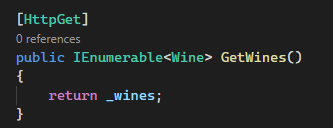
\includegraphics[width=0.5\textwidth]{controller-endpoint.png}
    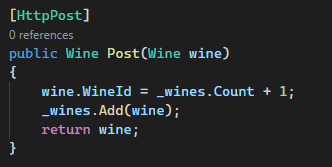
\includegraphics[width=0.4\textwidth]{controller-endpoint2.png}
    \caption{HTTP GET \& POST}
\end{figure}

\textbf{Route}

\begin{itemize}
    \item Een route is de URL naar het Endpoint
    \item Er zijn verschillende routes mogelijk per Endpoint
    \item Dezelfde routes zijn mogelijk zolang het HTTP Verb verschillend is
    \item We kunnen parameters megeven in de route via \{\}
    \item Indien geen routes: Default is GET met route = naam van Controller
\end{itemize}

\begin{figure}[H]
    \centering
    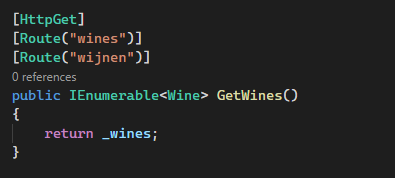
\includegraphics[width=0.45\textwidth]{controller-routes.png}
    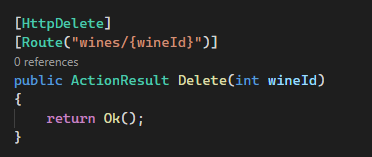
\includegraphics[width=0.5\textwidth]{controller-routes2.png}
    \caption{Meerdere routes per endpoint mogelijk (links). Delete request met parameters (rechts)}
\end{figure}

\begin{figure}[H]
    \centering
    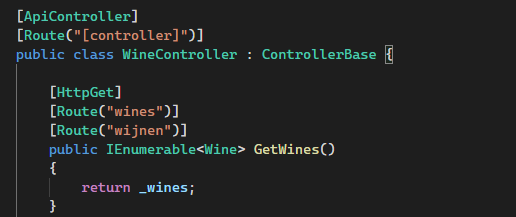
\includegraphics[width=0.5\textwidth]{controller-voorbeeld.png}
    \caption{\underline{https://localhost:5001/wine/wines} en \underline{https://localhost:5001/wine/wijnen}}
\end{figure}

\begin{figure}[H]
    \centering
    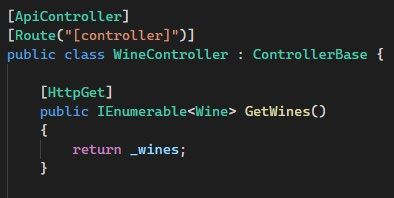
\includegraphics[width=0.4\textwidth]{controller-routes4.png}
    \caption{/wine haalt hij uit de naam WineController}
\end{figure}

\begin{figure}[H]
    \centering
    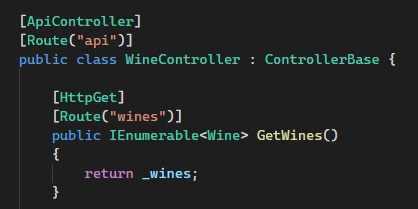
\includegraphics[width=0.5\textwidth]{controller-routes-api.png}
    \caption{Best practice: met api in de naam}
\end{figure}

\begin{figure}[H]
    \centering
    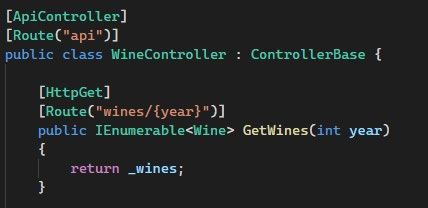
\includegraphics[width=0.5\textwidth]{controller-routes-parameter.png}
    \caption{Route met parameter. https://localhost:5001/api/wines/\textcolor{red}{2005}}
\end{figure}

\begin{itemize}
    \item Endpoints keren altijd iets terug:
    \begin{itemize}
        \item Status codes
        \item Data die we opvragen
    \end{itemize}
    \item Niet altijd makkelijk wat je moet kiezen
    \item Status codes uit HTTP standaard 5 grote verdelingen
\end{itemize}

\begin{figure}[H]
    \centering
    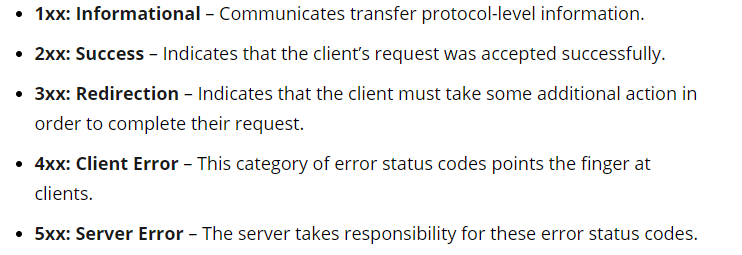
\includegraphics[width=0.5\textwidth]{http-statuscodes.png}
    \caption{Status codes}
\end{figure}

Overzicht statuscodes: \url{https://restfulapi.net/http-status-codes/}

Meest gebruikt: 

\begin{itemize}
    \item 200 OK
    \item 201 Created
    \item 400 Bad Request, 401 Unauthorized, 403 Forbidden, 415 Unsupported Media Type
    \item 500 Internal Server Error
\end{itemize}

\textbf{Returnen van data en statuscodes: veel ingebouwde klassen}

\begin{itemize}
    \item OkObjectResult(data)
    \item Ok()
    \item NotFoundObjectResult(data)
    \item NotFound()
    \item StatusCodeResult(int statuscode)
\end{itemize}

\subsection{Model binding}

\begin{itemize}
    \item Default enkel bij HTTP Post $\Rightarrow$
    \item ASP.NET Core volgorde voor ophalen van key/values:
    \begin{itemize}
        \item Form fields
        \item Request body (enkel bij gebruik [ApiController] attribuut)
        \item Route
        \item Querystring
    \end{itemize}
\end{itemize}

\subsubsection{Voorbeelden}

\begin{figure}[H]
    \centering
    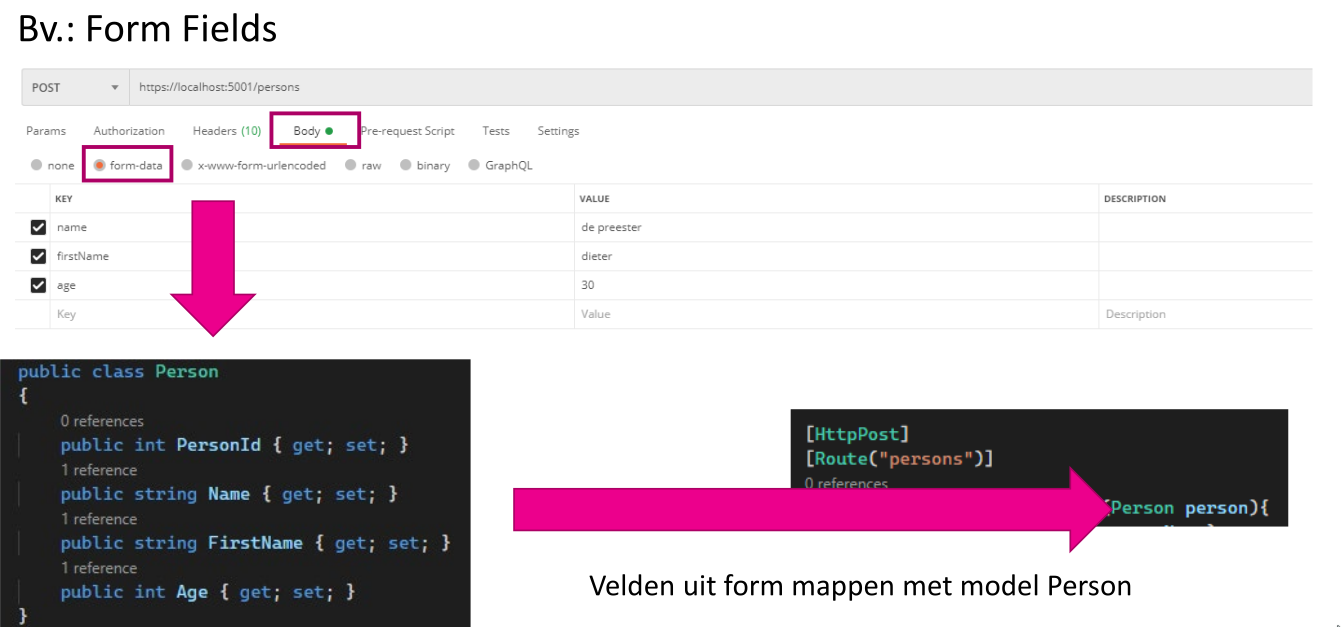
\includegraphics[width=0.5\textwidth]{model-binding-formfields.png}
    \caption{Voorbeeld: Form Fields}
\end{figure}

\begin{figure}[H]
    \centering
    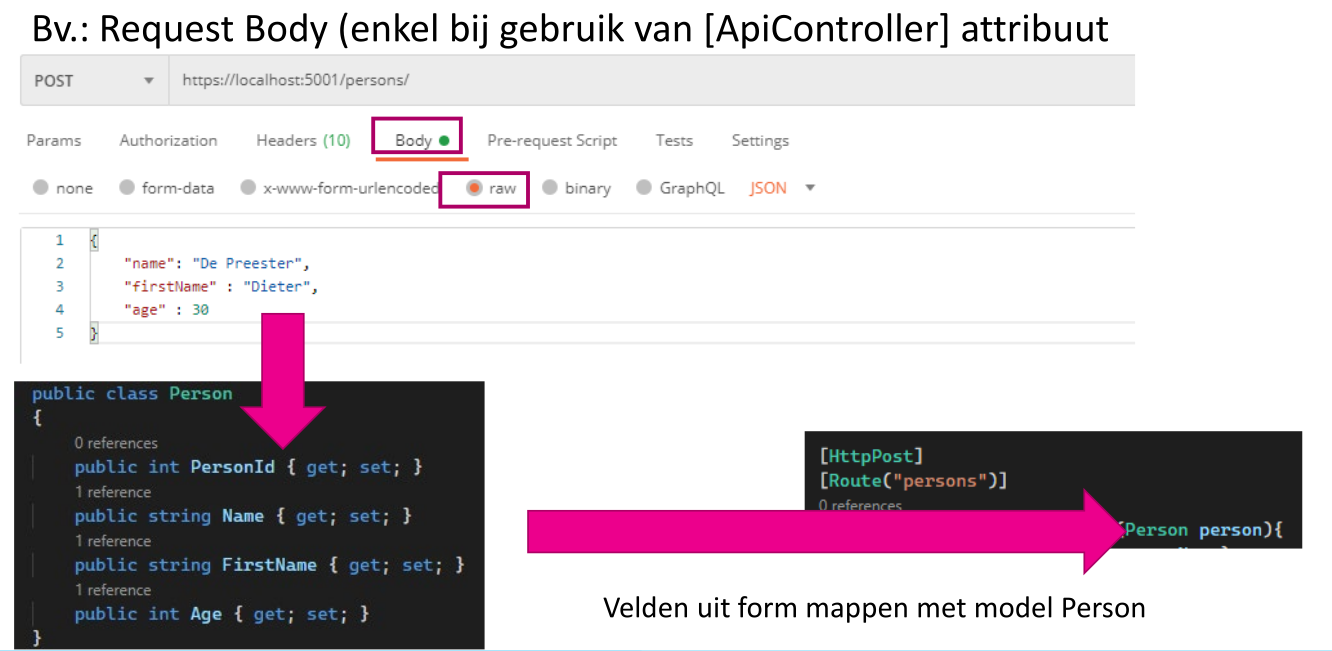
\includegraphics[width=0.5\textwidth]{model-binding-requestbody.png}
    \caption{Voorbeeld: Request Body (enkel bij gebruik van [ApiController] attribuut)}
\end{figure}

Via Route attribuut kunnen we parameters doorgeven:

\begin{figure}[H]
    \centering
    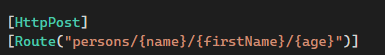
\includegraphics[width=0.5\textwidth]{model-binding-parameter.png}
    \caption{We bepalen de parameter namen tussen de \{parameter naam\}}
\end{figure}

\begin{figure}[H]
    \centering
    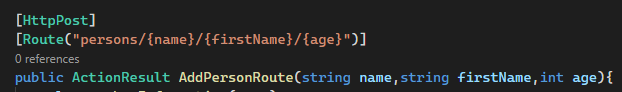
\includegraphics[width=0.5\textwidth]{model-binding-parameter2.png}
    \caption{In de C\# functie voorzien we dezelfde naam als in de route}
\end{figure}

\begin{figure}[H]
    \centering
    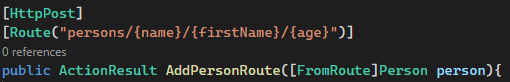
\includegraphics[width=0.5\textwidth]{model-binding-parameter3.png}
    \caption{We kunnen ook de waarden uit de route direct opslaan in het object: via \textbf{[FromRoute]} attribuut}
\end{figure}

\begin{figure}[H]
    \centering
    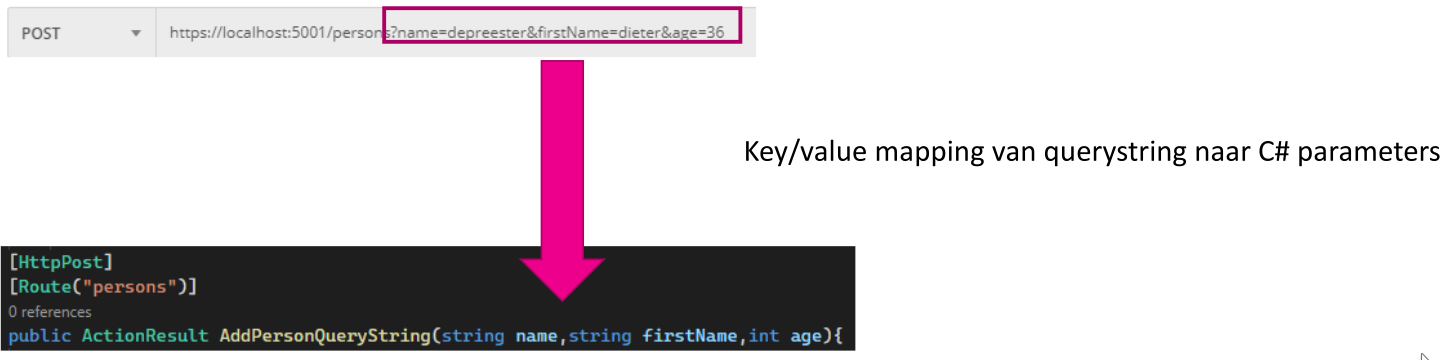
\includegraphics[width=0.5\textwidth]{model-binding-querystring.png}
    \caption{Kan ook via Querystring}
\end{figure}

\subsection{Configuration}

\begin{itemize}
    \item Bepaalde info willen we niet hardcoden
    \begin{itemize}
        \item Mailserver, connectionstring, password, \dots
    \end{itemize}
    \item We moeten dit buiten de applicatie kunnen opslaan (appsettings.json, Azure Keyvault)
\end{itemize}

\subsubsection{appsettings.json}

\begin{itemize}
    \item JSON file die bij de applicatie zit
    \item Verschillende versies mogelijk
    \begin{itemize}
        \item Development/Testing/Production..
    \end{itemize}
    \item Eerst geladen
    \item Bevat dingen die zowel voor development als production geldig zijn
    \item appsettings.Development.json (naargelang de omgeving inladen)
    \begin{itemize}
        \item Overriden wat reeds in appsettings.json szit
    \end{itemize}
    \item JSON file
\end{itemize}

\begin{figure}[H]
    \centering
    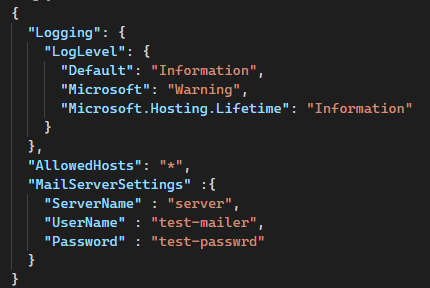
\includegraphics[width=0.5\textwidth]{appsettings-json.png}
    \caption{Probeer met Secties te werken (zie MailServerSettings)}
\end{figure}

\begin{itemize}
    \item We gebruiken Option pattern voor inladen data uit configuratie files
    \item Eerst klasse maken die overeenkomt met de waarden in de JSON file
\end{itemize}

\begin{figure}[H]
    \centering
    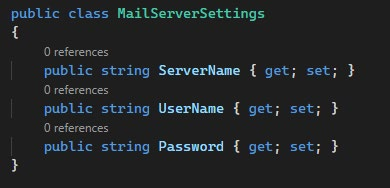
\includegraphics[width=0.5\textwidth]{appsettings-json-secties.png}
    \caption{Klasse die overeenkomt met het MailServerSettings object in appsettings.json}
\end{figure}

\begin{itemize}
    \item Registreren van de sectie in de startup en koppelen aan de klasse
    \item Hierdoor krijgen we een strongly typed settings file
\end{itemize}

\begin{figure}[H]
    \centering
    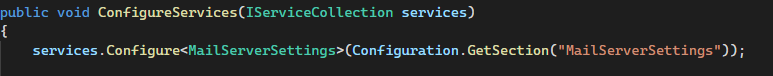
\includegraphics[width=0.6\textwidth]{appsettings-json-configure.png}
    \caption{Configuration.GetSection("SectionNaam")}
\end{figure}

Gebruik in de controller: 

\begin{itemize}
    \item IOptions<MailServerSettings> via CONSTRUCTOR (CTOR) binnenbrengen
    \item Value property zal deze uitlezen en opslaan in property \_mailserverSettings
    \item Hierdoor kunnen we deze vlot uitlezen in de controller en gebruiken
\end{itemize}

\begin{figure}[H]
    \centering
    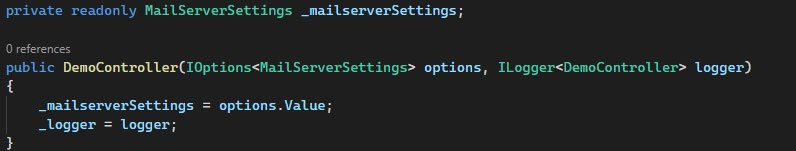
\includegraphics[width=0.5\textwidth]{appsettings-json-controller.png}
    \caption{}
\end{figure}

In VSCode:

\begin{itemize}
    \item launch.json openen
    \item Hier kan je de profielen vinden
    \item Copy/paste profile
    \item Per profiel kan je instellingen maken zoals URL of ASPNETCORE\_ENVIRONMENT
\end{itemize}

\begin{figure}[H]
    \centering
    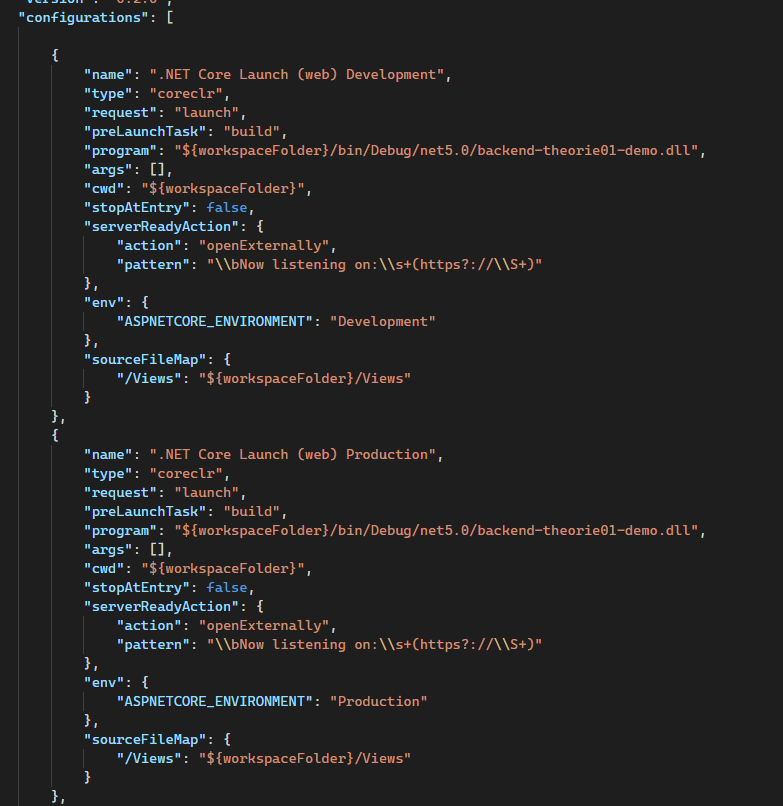
\includegraphics[width=0.3\textwidth]{appsettings-json-vscode.png}
    \caption{launch.json}
\end{figure}

\begin{figure}[H]
    \centering
    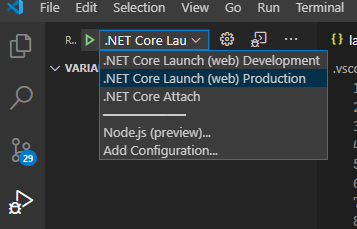
\includegraphics[width=0.3\textwidth]{appsettings-json-vscode2.png}
    \caption{In de dropdown kies je wat je wil starten}
\end{figure}


\textbf{Visual Studio 2019}

\begin{itemize}
    \item We bepalen de profielen in de map Properties
    \item In launchSettings.json
\end{itemize}

\subsubsection{Azure Keyvault}

\begin{itemize}
    \item Kluis in Azure waar alle info zit
    \item Beste oplossing voor productie projecten
\end{itemize}

\subsection{Wat moet je kennen?}

\begin{itemize}
    \item Zorg dat je de HTTP Request/Response kan uitleggen
    \item Wat zijn statuscodes en wanneer gebruik ik welke
    \item Een duidelijke API URL kunnen opstellen
    \item Manieren van modelbinding
    \item Hoe configureer je uw omgeving met profielen
\end{itemize}

\end{document}